\documentclass{beamer}
\beamertemplatenavigationsymbolsempty
\usecolortheme{beaver}
\setbeamertemplate{blocks}[rounded=true, shadow=true]
\setbeamertemplate{footline}[page number]
%
\usepackage[utf8]{inputenc}
\usepackage[english,russian]{babel}
\usepackage{amssymb,amsfonts,amsmath,mathtext,amsthm,mathtools}
\usepackage{algorithm}
\usepackage{algpseudocode}
\usepackage{subfig}
\usepackage[all]{xy} % xy package for diagrams
\usepackage{array}
\usepackage{multicol}% many columns in slide
\usepackage{hyperref}% urls
\usepackage{hhline}%tables
% Your figures are here:
\graphicspath{ {fig/} {../fig/} }

%----------------------------------------------------------------------------------------------------------
\title[\hbox to 56mm{Стохастический метод Ньютона}]{Стохастический метод Ньютона \\ с различным семплингом}
\author{Денис Швейкин}
\institute{Московский физико-технический институт}
\date{\footnotesize
\par\smallskip\emph{Курс:} Моя первая научная статья
\par\smallskip\emph{Эксперт:} Рустем Исламов
\par\bigskip\small 2023}
%----------------------------------------------------------------------------------------------------------
\begin{document}
%----------------------------------------------------------------------------------------------------------
\begin{frame}
\thispagestyle{empty}
\maketitle
\end{frame}
%-----------------------------------------------------------------------------------------------------
\begin{frame}{Цель исследования}
	
\begin{block}{Задача}
	Использовать различные стратегии семплинга для стохастического метода Ньютона, чтобы получить наилучшую скорость сходимости
\end{block}

\begin{block}{Мотивация}
	\begin{itemize}
		\item Задача минимизации функции потерь, имеющей структуру конечной суммы, возникает повсеместно в машинном обучении. Методы первого порядка для этой задачи хорошо изучены
		\item Методы второго порядка типа Ньютон лучше адаптируются к кривизне задачи и имеют квадратичную сходимость. Однако эти методы изучены менее подробно
		\item Применяются различные стратегии семплинга для стохастического варианта, поскольку для методов первого порядка их подбор ведет к улучшеням скорости сходимости
	\end{itemize}
\end{block}

\end{frame}
%-----------------------------------------------------------------------------------------------------
\begin{frame}{Минимизируемая функция}


	\begin{block}{Структура функции потерь}
	$$\underset{x \in \mathbb R^d}{\min} \left[ f(x) \overset{def}{=} \frac{1}{n} \sum \limits_{i=1}^n f_i(x) \right]$$
	\end{block}

	\begin{block}{Предположения}
	\begin{itemize}
   	\item Сильная выпуклость
   	$$f(x) \geqslant f(y) + \langle \nabla f, x - y \rangle + \frac{\mu}{2} \| x - y \|^2$$
   	\item Липшицевы Гессианы
   	$$\| \nabla^2 f(x) - \nabla^2 f(y) \| \leqslant H \| x - y \|$$
	\end{itemize}
\end{block}

\bigskip

\end{frame}


%----------------------------------------------------------------------------------------------------------
\begin{frame}{Алгоритм}

	\begin{algorithmic}
		\item \textbf{Initialize:} Задать начальные приближения $w_1^0, w_2^0, ... w_n^0 \in \mathbb R^d$
		
		\item \For {$k = 0, 1, 2, ...$}	
		
		$ x^{k+1} = \left[ \frac{1}{n} \sum \limits_{i=1}^n \nabla^2 f_i(w_i^k) \right]^{-1} \left[ \frac{1}{n} \sum \limits_{i=1}^n \nabla^2 f_i(w_i^k) w_i^k - \nabla f_i(w_i^k) \right] $
		
		Выбрать множество $S^k \subseteq \{ 1, 2, ..., n \}$ одной из стратегий семплинга
		
		$w_i^{k+1} = 
		\begin{cases}
			x^{k+1} & i \in S^k \\
			w_i^k & i \notin S^k
		\end{cases}$
		
		\item \EndFor
	\end{algorithmic}
	
	\begin{block}{Определение}
	Семплингом называется $\hat S: [n] \rightarrow 2^{[n]}$ 
	\end{block}

	\begin{block}{Метрика качества}
		Качество стратегий измеряется в скорости сходимости
	\end{block}

\end{frame}
%----------------------------------------------------------------------------------------------------------
\begin{frame}{Стратегии семплинга}
	
	\begin{block}{Определение}
		Семплингом называется $\hat S: [n] \rightarrow 2^{[n]}$ 
	\end{block}
	
\begin{columns}[c]
\column{0.5\textwidth}
    \begin{block}{Однородные стратегии}	
    	Любое множество размера $j$ выбирается с одинаковой вероятностью, $P(|\hat S| = j) = q_j$
    	Пример: $\tau$-nice семплинг \\
    		$$ q_\tau = 1 $$
    \end{block}
	\begin{block}{Независимые стратегии}
		Теперь каждый объект $i$ включается в множество $S$ независимо с вероятностью $p_i$.
	\end{block}
\column{0.5\textwidth}
    \begin{block}{Importance sampling}
    	Каждая $f_i$ имеет свою константу Липшица $H_i$
    	$$p_i = \frac{H_i}{\sum \limits_{i=1}^n H_i}$$
    \end{block}
	\begin{block}{Последовательная стратегия}
		Проходить по данным в порядке, заданном случайное перестановкой
	\end{block}
\end{columns}

\end{frame}
%----------------------------------------------------------------------------------------------------------
\begin{frame}{Результаты: оценки скорости сходимости}
	
\begin{columns}[c]
\column{0.5\textwidth}
	\begin{block}{Средний квадрат незвяки}
		$\mathcal W^k \overset{\text{def}} = \frac{1}{n} \sum \limits_{i=1}^n \| w_i^k - x^* \|^2$
	\end{block}
	\begin{block}{Однородные стратегии}
		Пусть $p = \frac{\mathbb E[|\hat S|]}{n}$. Тогда \\
		$ \mathbb E_k[\mathcal W^{k+1}] \leqslant \left( 1 - \frac{3}{4}p \right) \mathcal W^k$ \\
		Результат получается одинаковым для любой стратегии. Поэтому при равных $p$ различие будет только в удобстве реализаций стратегий
	\end{block}
\column{0.5\textwidth}
	\begin{block}{Независимые стратегии}
		Пусть фиксировано матожидание размера батча $\mathbb E_k[|\hat S^k|] = \tau$. Тогда	$ \mathbb E_k[\mathcal W^{k+1}] $ будет минимально, если некоторые $p_i$ равны 1, возможно одно $p_i \in(0,1)$, а остальные равны $0$. "Аппроксимируется" последовательной стратегией
	\end{block}

	\begin{block}{Importance sampling}
		Теоретических гарантий сходимости нет
	\end{block}

\end{columns}
	
\end{frame}
%----------------------------------------------------------------------------------------------------------
\begin{frame}{Вычислительный эксперимент}

\begin{columns}[c]
	\column{0.5\textwidth}
		\begin{enumerate}
			\item Однородные стратегии $\rightarrow$
			\item Importance sampling $\searrow$
			\item Последовательная стратегия $\downarrow$
		\end{enumerate}
		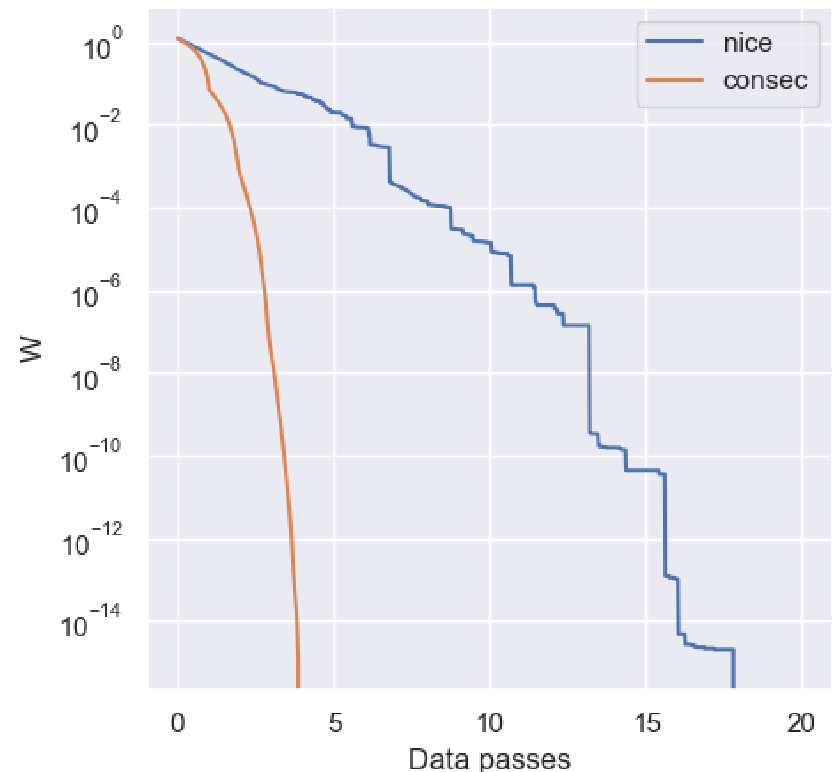
\includegraphics[width=0.8\textwidth]{consecutive strategy 10}
	\column{0.4\textwidth}
		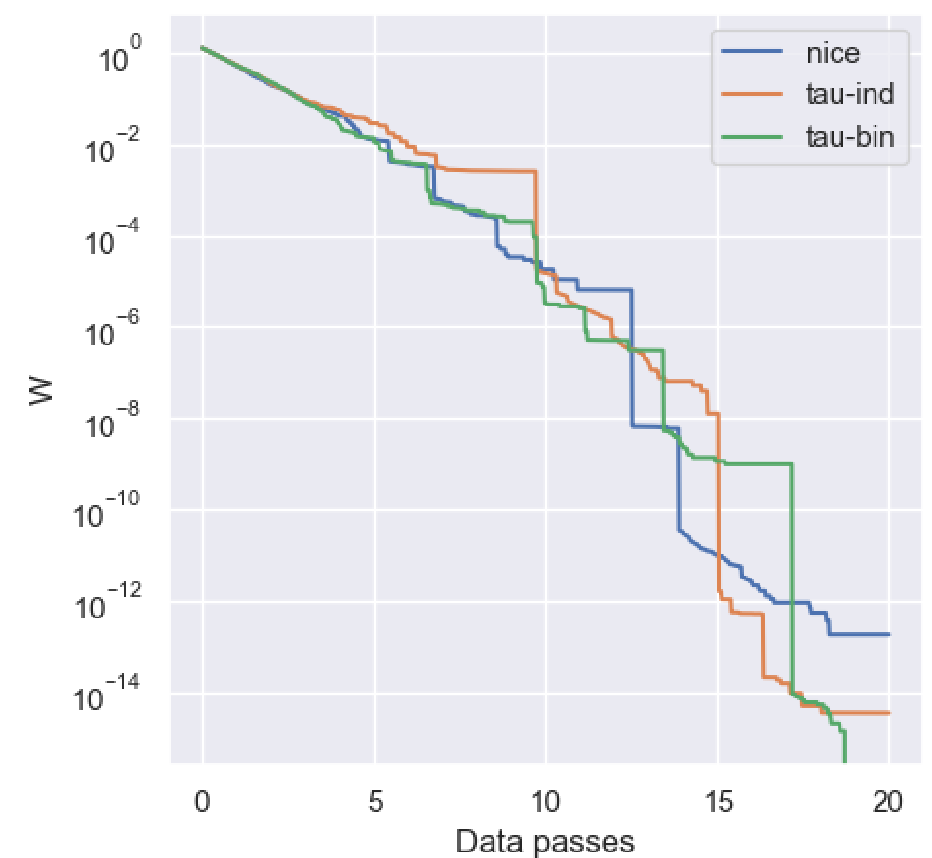
\includegraphics[width=\textwidth]{uniform strategies}
		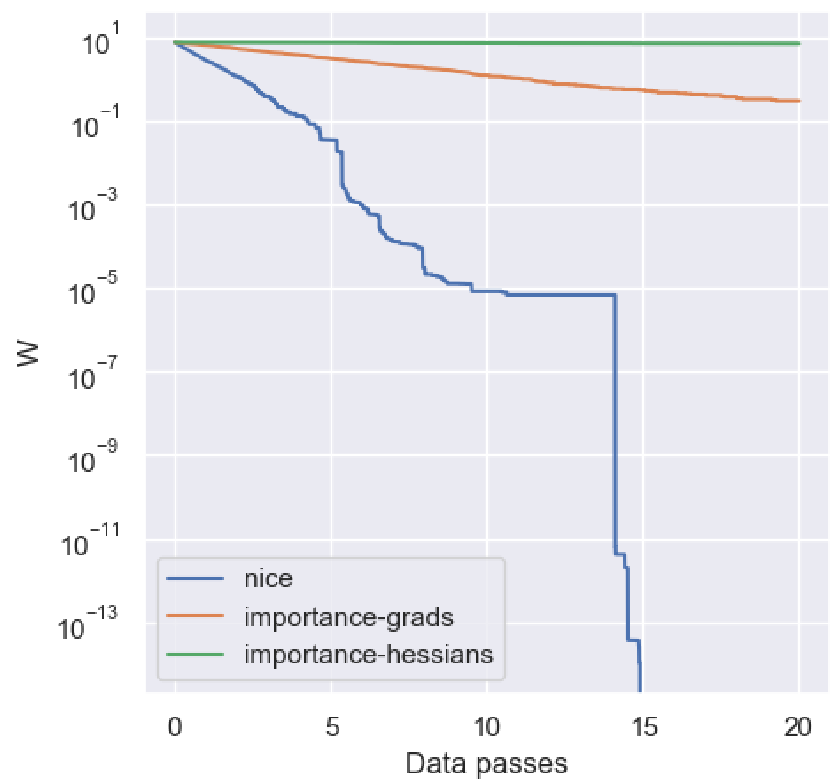
\includegraphics[width=\textwidth]{importance sampling}
\end{columns}

\end{frame}
%----------------------------------------------------------------------------------------------------------
\begin{frame}{Заключение}
    \begin{block}{}
    \begin{itemize}
        \item Получены линейные оценки скорости сходимости для однородных стратегий в общем случае. Показана практическая эквивалентность основных вариантов однородных стратегий
        \item Для Importance sampling теоретических гарантий сходимости нет, и в эксперименте он уступает базовому методу $\tau$-nice
        \item Последовательная стратегия показывает себя лучше. Тем не менее, теоретическое обоснование нужно уточнять и улучшать в дальнейшем
    \end{itemize}
    \end{block}
\end{frame}
%----------------------------------------------------------------------------------------------------------
\end{document} 